% This LaTeX was auto-generated from MATLAB code.
% To make changes, update the MATLAB code and export to LaTeX again.

\documentclass{article}

\usepackage[utf8]{inputenc}
\usepackage[T1]{fontenc}
\usepackage{lmodern}
\usepackage{graphicx}
\usepackage{color}
\usepackage{listings}
\usepackage{hyperref}
\usepackage{amsmath}
\usepackage{amsfonts}
\usepackage{epstopdf}
\usepackage{matlab}

\sloppy
\epstopdfsetup{outdir=./}
\graphicspath{ {./draft2_images/} }

\begin{document}

\matlabtitle{RX vs SSRX}

\begin{par}
\begin{flushleft}
Doron Serebro 07.05.2020
\end{flushleft}
\end{par}

\vspace{1em}

\matlabheading{Introduction}

\begin{par}
\begin{flushleft}
This notebook a working draft for the course project on the topic of "comparing RX and SSRX algorithms". The goal is to run RX and SSRX on the same dataset, find the differences and try to explain them in a meaningful way.
\end{flushleft}
\end{par}

\begin{par}
\begin{flushleft}
For now, this project is implemented on the RIT Blind Test data set.
\end{flushleft}
\end{par}


\matlabheading{RX Algorithm}

\begin{par}
\begin{flushleft}
The RX algorithm is given by: $\textrm{RX}={\left(\overrightarrow{X} -\overrightarrow{m} \right)}^T \phi^{-1} \left(\overrightarrow{X} -\overrightarrow{m} \right)>\mathrm{Threshold}$. 
\end{flushleft}
\end{par}

\begin{par}
\begin{flushleft}
The threshold used in this implementation is  3-sigma: $\eta =\mu +3\sigma$, whre $\mu \;$is the mean RX score and $\sigma$ is the standard devation of the RX scores.
\end{flushleft}
\end{par}

\begin{matlabcode}
file = 'G:\My Drive\Project\self_test\HyMap\self_test_rad.img';
[mat,hdr] = auto_load_HS(file);
\end{matlabcode}
\begin{matlaboutput}
Loading ENVI header ...
Loading ENVI image ...
\end{matlaboutput}
\begin{matlabcode}
data=double(permute(mat,[2,1,3]));
[x_size,y_size, num_of_bands]=size(data);
[X_MINUS_M,phi]=HSI_MF_params(data);
phi_inv = pinv(phi);
RX = zeros(x_size,y_size);
for x = 1:x_size
    for y = 1:y_size
        x_minus_m = squeeze(X_MINUS_M(x,y,:));
        RX(x,y) = x_minus_m' * phi_inv * x_minus_m;
    end
end
RX= RX';
RX_filt = RX > mean(RX(:)) + 3*std(RX(:));
\end{matlabcode}


\matlabheading{SSRX Algorithm}

\begin{par}
\begin{flushleft}
The SSRX algorithm adds a preprocessing step to the RX algrotihm - performing PCA and keeping only low variance PCs.
\end{flushleft}
\end{par}

\begin{par}
\begin{flushleft}
the formula for PCA is given by: 
\end{flushleft}
\end{par}

\begin{par}
$$X_{\mathrm{PCA}} =\left(X-m\right)\phi {\;}^{-1} V_q$$
\end{par}

\begin{par}
$$\begin{array}{l}\linebreak 
m-\textrm{the}\;\textrm{per}\;\textrm{channel}\;\textrm{mean}\;\textrm{of}\;X\\\linebreak 
\phi -\textrm{the}\;\textrm{covariance}\;\textrm{matrix}\\\linebreak 
V_q -a\;\textrm{matrix}\;\textrm{where}\;\textrm{every}\;\textrm{column}\;\textrm{is}\;\textrm{an}\;\textrm{eigen}\;\textrm{vector}\;\textrm{of}\;\phi \;\mathrm{while}\;\mathrm{ommiting}\;\mathrm{the}\;q\;\mathrm{eigen}\;\mathrm{vectors}\;\mathrm{that}\;\mathrm{correspond}\;\mathrm{to}\;\mathrm{the}\;\mathrm{highest}\;\mathrm{variance}\;\mathrm{eigen}\;\mathrm{values}\linebreak 
\end{array}$$
\end{par}

\begin{matlabcode}
q = 120;
[V, D] = eigs(phi,126);
V2 = V(:,3:end);% deleting first 2 PC
V4 = V(:,5:end);% deleting first 4 PC
V6 = V(:,7:end);% deleting first 6 PC
data_pca2D2 = reshape(X_MINUS_M,x_size*y_size,num_of_bands) * V2;
data_pca2D4 = reshape(X_MINUS_M,x_size*y_size,num_of_bands) * V4;
data_pca2D6 = reshape(X_MINUS_M,x_size*y_size,num_of_bands) * V6;

data_pca2   = hyperConvert3d(data_pca2D2', x_size,y_size,num_of_bands);
data_pca4  = hyperConvert3d(data_pca2D4', x_size,y_size,num_of_bands);
data_pca6 = hyperConvert3d(data_pca2D6', x_size,y_size,num_of_bands);

\end{matlabcode}

\begin{par}
\begin{flushleft}
Now that we have the preprocessed data, we can run the RX algorithm on it to get SSRX:
\end{flushleft}
\end{par}

\begin{matlabcode}
%calc phi_inv
[X_MINUS_M_PCA2,phi_pca2]=HSI_MF_params(data_pca2);
[X_MINUS_M_PCA4,phi_pca4]=HSI_MF_params(data_pca4);
[X_MINUS_M_PCA6,phi_pca6]=HSI_MF_params(data_pca6);

phi_pca_inv2 = pinv(phi_pca2);
phi_pca_inv4 = pinv(phi_pca4);
phi_pca_inv6 = pinv(phi_pca6);

%init empty results matrices
SSRX2   = zeros(x_size,y_size);
SSRX4  = zeros(x_size,y_size);
SSRX6 = zeros(x_size,y_size);

for x = 1:x_size
    for y = 1:y_size
        x_minus_m2 = squeeze(X_MINUS_M_PCA2(x,y,:));
        x_minus_m4 = squeeze(X_MINUS_M_PCA4(x,y,:));
        x_minus_m6 = squeeze(X_MINUS_M_PCA6(x,y,:));
        
        SSRX2(x,y) = x_minus_m2' * phi_pca_inv2 * x_minus_m2;
        SSRX4(x,y) = x_minus_m4' * phi_pca_inv4 * x_minus_m4;      
        SSRX6(x,y) = x_minus_m6' * phi_pca_inv6 * x_minus_m6;
    end
end
SSRX2= SSRX2';
SSRX4= SSRX4';
SSRX6= SSRX6';
SSRX2_filt = SSRX2 > mean(SSRX2(:)) + 3*std(SSRX2(:));
SSRX4_filt = SSRX4 > mean(SSRX4(:)) + 3*std(SSRX4(:));
SSRX6_filt = SSRX6 > mean(SSRX6(:)) + 3*std(SSRX6(:));
\end{matlabcode}


\matlabheading{Scatter Plot Comparison}

\begin{par}
\begin{flushleft}
Based on the results above, the difference between the 2 algorithms (if exists) is in the lower scored anomalies. Let's try to look at that:
\end{flushleft}
\end{par}

\begin{matlabcode}
h1=figure; 
spy(RX_filt,'or'); 
hold on;
spy(SSRX2_filt,'xg');
legend('RX','SSRX2');
title('RX vs SSRX (deleting 2 highest variance PCs');
set(h1, 'Position', [0 0 1200 600])
\end{matlabcode}
\begin{center}
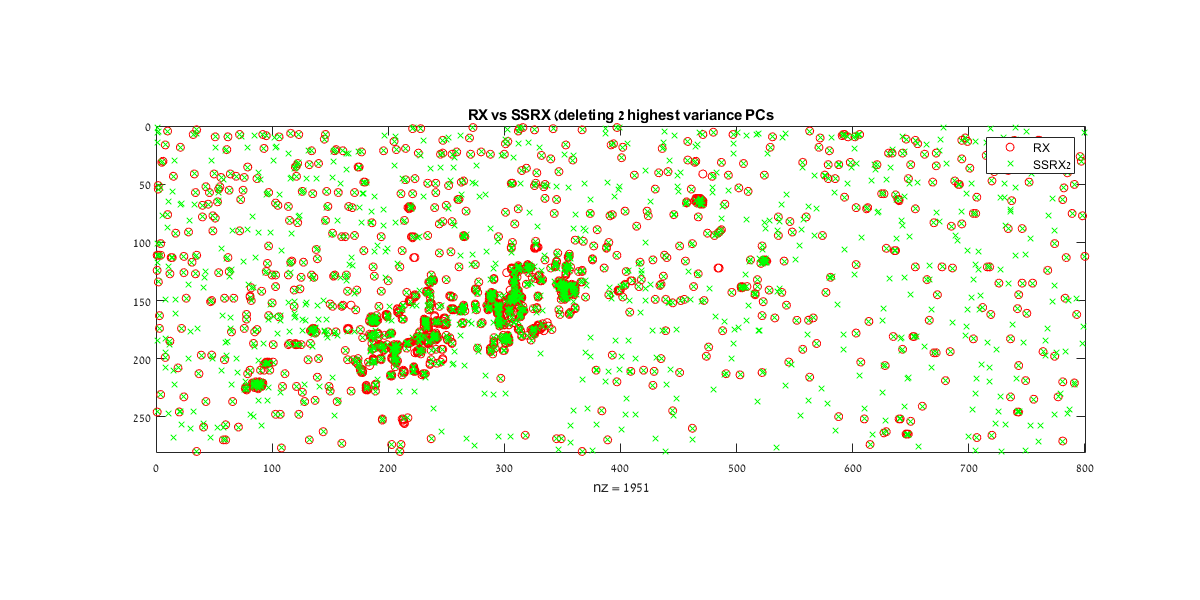
\includegraphics[width=\maxwidth{120.42147516307075em}]{figure_0}
\end{center}
\begin{matlabcode}
h2=figure; 
spy(RX_filt,'or'); 
hold on;
spy(SSRX4_filt,'xg');
legend('RX','SSRX4');
title('RX vs SSRX (deleting 4 highest variance PCs');
set(h2, 'Position', [0 0 1200 600])
\end{matlabcode}
\begin{center}
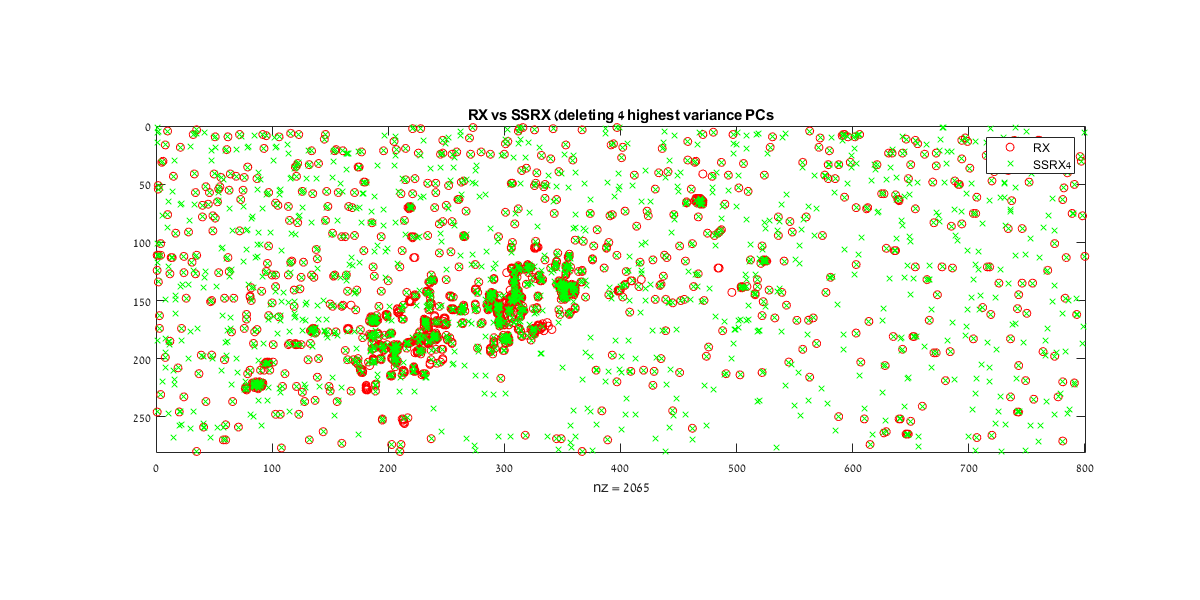
\includegraphics[width=\maxwidth{120.42147516307075em}]{figure_1}
\end{center}
\begin{matlabcode}
h3=figure; 
spy(RX_filt,'or'); 
hold on;
spy(SSRX6_filt,'xg');
legend('RX','SSRX6');
title('RX vs SSRX (deleting 6 highest variance PCs');
set(h3, 'Position', [0 0 1200 600])
\end{matlabcode}
\begin{center}
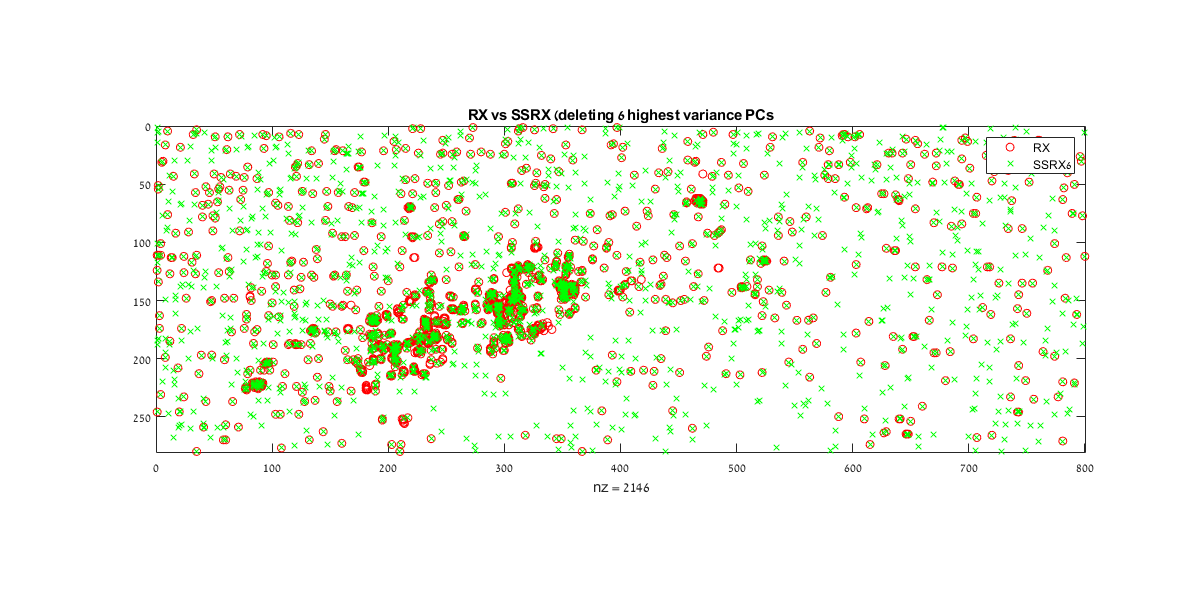
\includegraphics[width=\maxwidth{120.42147516307075em}]{figure_2}
\end{center}

\begin{par}
\begin{flushleft}
\textbf{Conclusion:} The number of anomalies detected is increased with every PC removed.
\end{flushleft}
\end{par}


\matlabheading{Anomalies Gained by SSRX}

\begin{par}
\begin{flushleft}
In order to characterize the difference in anomalies, let's examine what new anomalies were detected in the SSRX algorithm, but not in the RX algorithm.
\end{flushleft}
\end{par}

\begin{par}
\begin{flushleft}
number of anomalies SSRX2 detected that RX did not:
\end{flushleft}
\end{par}

\begin{matlabcode}
SSRX2_miss = SSRX2_filt.*(1-RX_filt);
% sum(nonzeros(SSRX2_diff))
h3=figure; 
imshow(data(:,:,1)',[]);
hold on;
spy(SSRX2_miss,'xr');
title('Anomalies Unique to SSRX2');
set(h3, 'Position', [0 0 1200 600])
\end{matlabcode}
\begin{center}
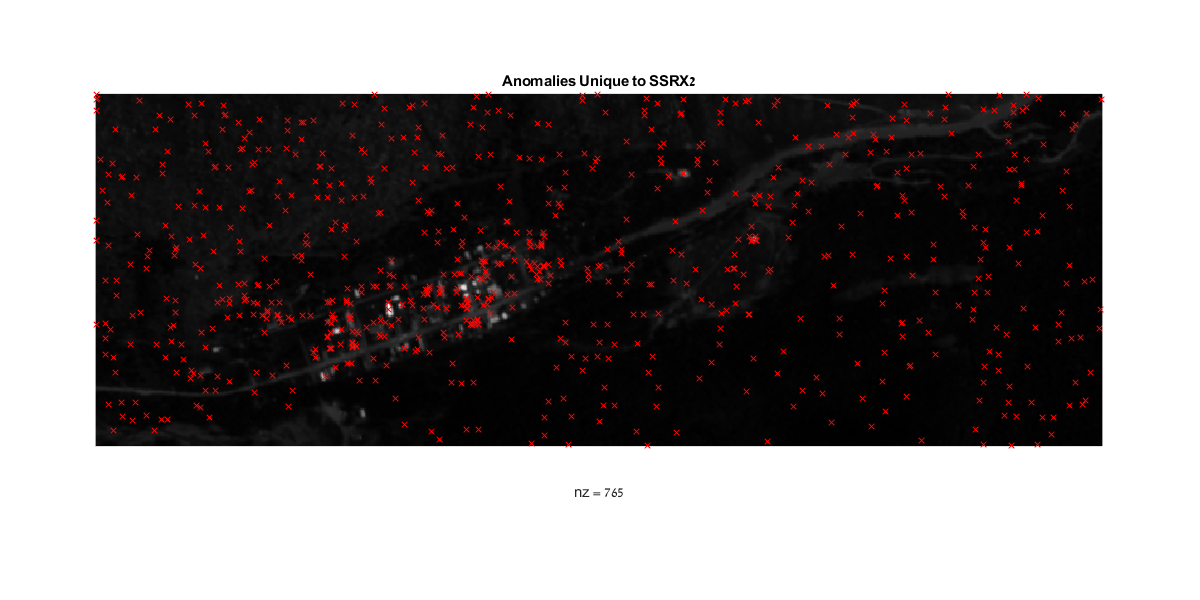
\includegraphics[width=\maxwidth{120.42147516307075em}]{figure_3}
\end{center}

\vspace{1em}

\begin{par}
\begin{flushleft}
number of anomalies SSRX4 detected that RX did not:
\end{flushleft}
\end{par}

\begin{matlabcode}
SSRX4_diff = SSRX4_filt.*(1-RX_filt);
% sum(nonzeros(SSRX4_diff))
h3=figure; 
 imshow(data(:,:,1)',[]);
hold on;
spy(SSRX4_diff,'xg');
title('Anomalies Unique to SSRX4');
set(h3, 'Position', [0 0 1200 600])
\end{matlabcode}
\begin{center}
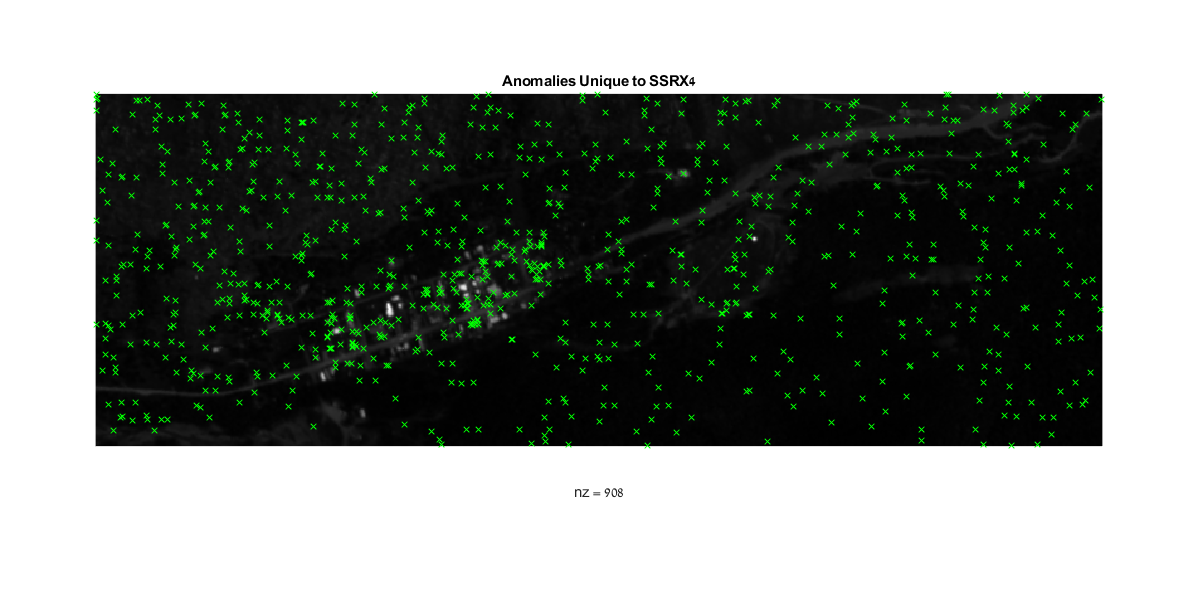
\includegraphics[width=\maxwidth{120.42147516307075em}]{figure_4}
\end{center}

\begin{par}
\begin{flushleft}
number of anomalies SSRX6 detected that RX did not:
\end{flushleft}
\end{par}

\begin{matlabcode}
SSRX6_diff = SSRX6_filt.*(1-RX_filt);
% sum(nonzeros(SSRX6_diff))
h3=figure; 
 imshow(data(:,:,1)',[]);
hold on;
spy(SSRX6_diff,'xb');
title('Anomalies Unique to SSRX6');
set(h3, 'Position', [0 0 1200 600])
\end{matlabcode}
\begin{center}
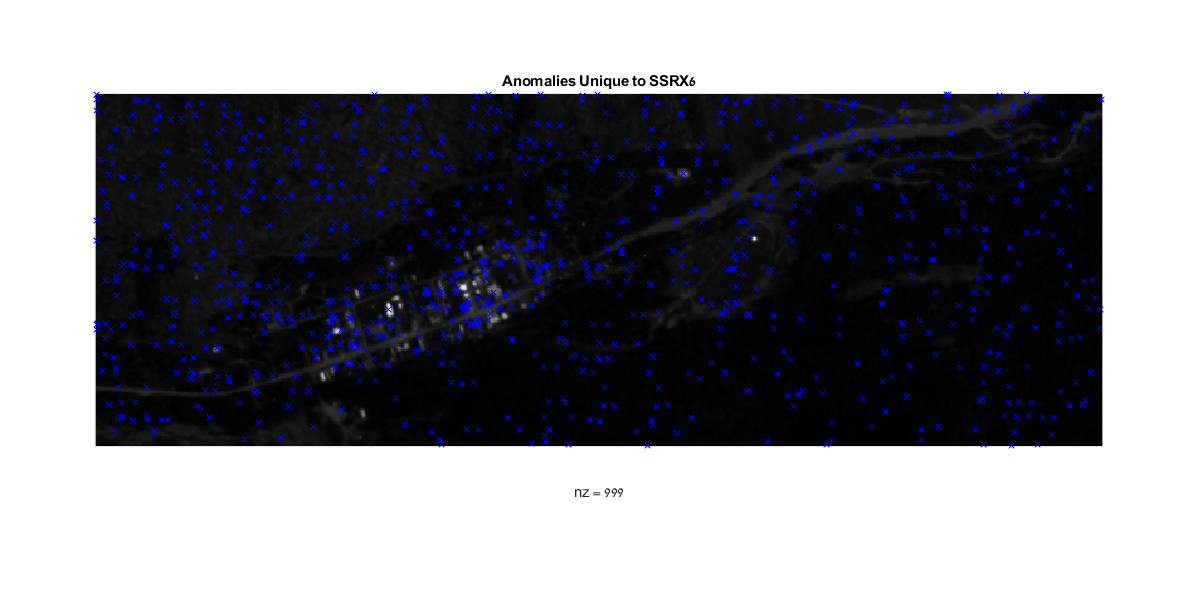
\includegraphics[width=\maxwidth{120.42147516307075em}]{figure_5}
\end{center}

\begin{par}
\begin{flushleft}
Conclusion: the more PCs we drop, the more noisy anomalies we get.
\end{flushleft}
\end{par}


\matlabheading{Anomalies Missed by SSRX}

\begin{par}
\begin{flushleft}
Let's examine 
\end{flushleft}
\end{par}

\begin{matlabcode}
SSRX2_miss = (1-SSRX2_filt).*RX_filt;
% sum(nonzeros(SSRX2_diff))
h3=figure; 
imshow(data(:,:,1)',[]);
hold on;
spy(SSRX2_miss,'xr');
title('Anomalies Missed by SSRX2');
set(h3, 'Position', [0 0 1200 600])
\end{matlabcode}
\begin{center}
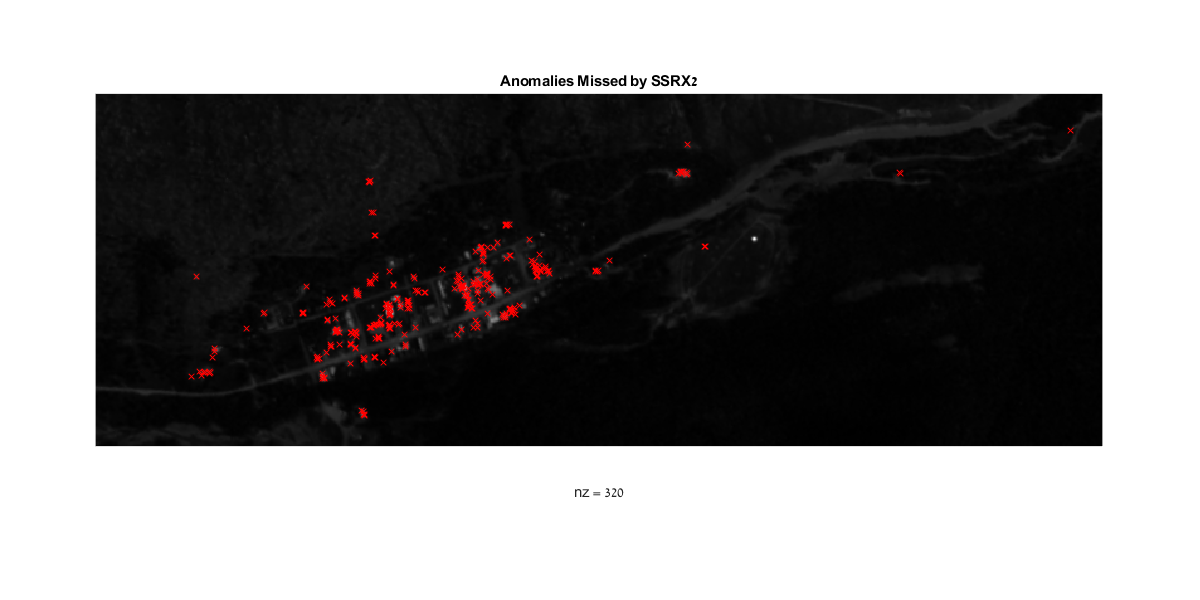
\includegraphics[width=\maxwidth{120.42147516307075em}]{figure_6}
\end{center}

\vspace{1em}

\begin{par}
\begin{flushleft}
number of anomalies SSRX4 detected that RX did not:
\end{flushleft}
\end{par}

\begin{matlabcode}
SSRX4_miss = (1-SSRX4_filt).*RX_filt;
% sum(nonzeros(SSRX4_diff))
h3=figure; 
 imshow(data(:,:,1)',[]);
hold on;
spy(SSRX4_miss,'xg');
title('Anomalies Missed by SSRX4');
set(h3, 'Position', [0 0 1200 600])
\end{matlabcode}
\begin{center}
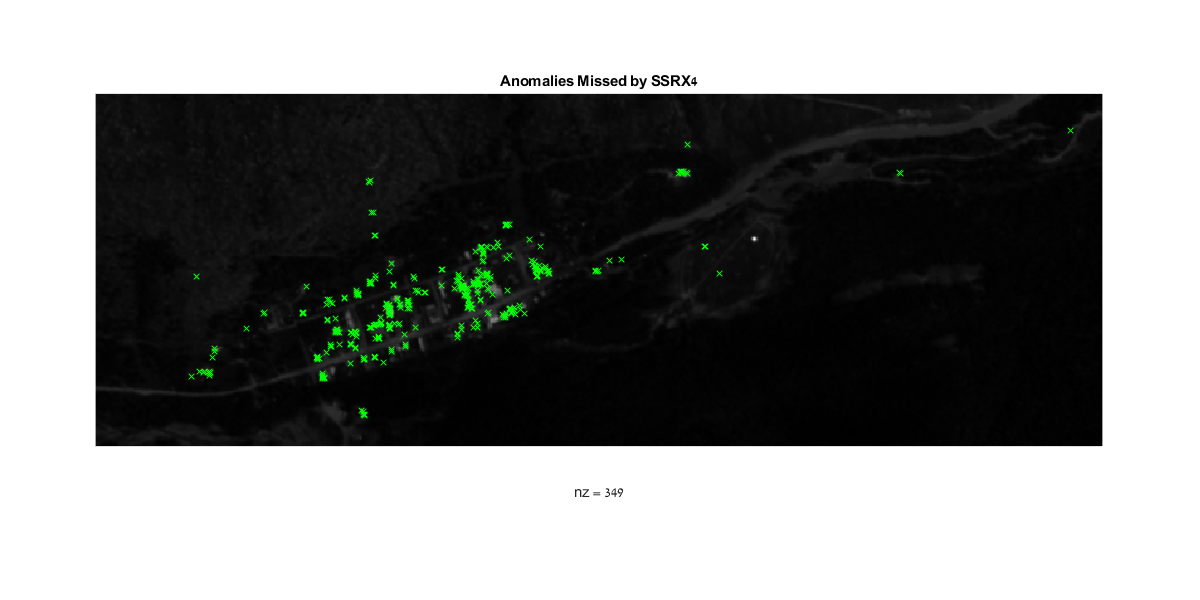
\includegraphics[width=\maxwidth{120.42147516307075em}]{figure_7}
\end{center}

\begin{par}
\begin{flushleft}
number of anomalies SSRX6 detected that RX did not:
\end{flushleft}
\end{par}

\begin{matlabcode}
SSRX6_miss = (1-SSRX6_filt).*RX_filt;
% sum(nonzeros(SSRX6_diff))
h3=figure; 
 imshow(data(:,:,1)',[]);
hold on;
spy(SSRX6_miss,'xb');
title('Anomalies Missed by SSRX6');
set(h3, 'Position', [0 0 1200 600])
\end{matlabcode}
\begin{center}
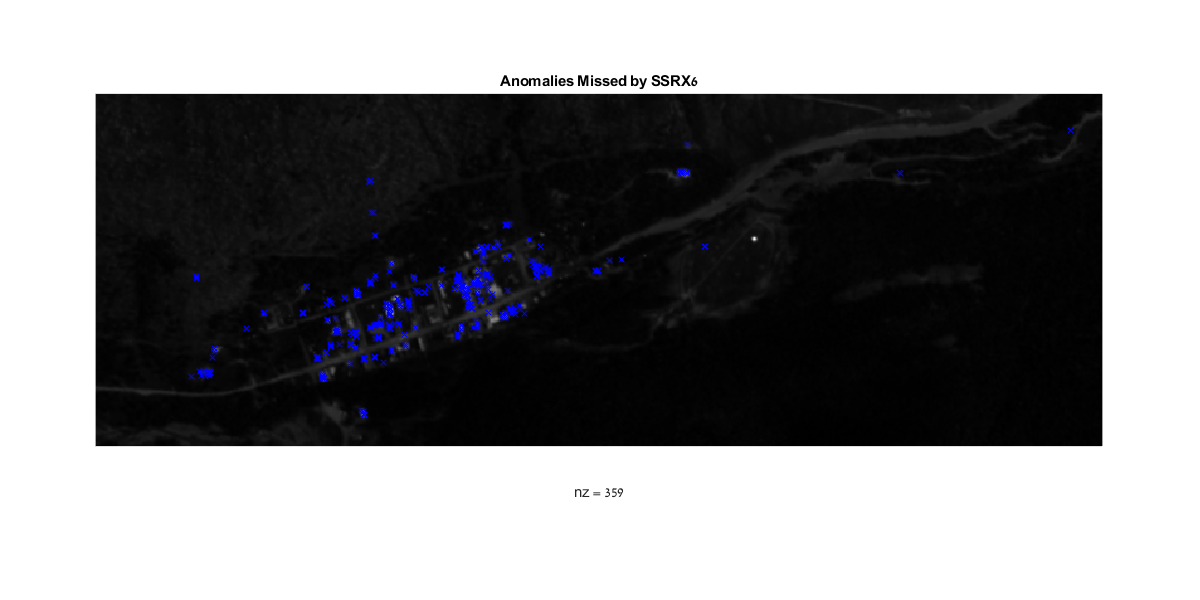
\includegraphics[width=\maxwidth{120.42147516307075em}]{figure_8}
\end{center}
\begin{matlabcode}
[RX_val,RX_bins]=histcounts(RX,1000);
[SSRX2_val,SSRX2_bins]=histcounts(SSRX2,1000);
% [SSRX4_val,SSRX4_bins]=histcounts(SSRX4,1000);
% [SSRX6_val,SSRX6_bins]=histcounts(SSRX6,1000);
figure;
plot(RX_bins(1:1000),RX_val);
hold on;
plot(SSRX2_bins(1:1000),SSRX2_val);
% plot(SSRX4_bins(1:1000),SSRX4_val);
% plot(SSRX6_bins(1:1000),SSRX6_val);
xlim([-100 1000]);
legend('RX','SSRX2');
title('Histograms');
\end{matlabcode}
\begin{center}
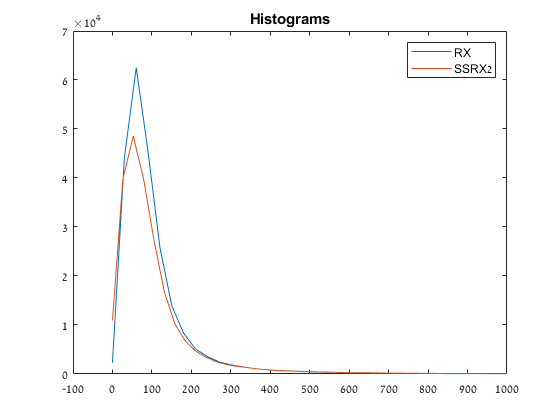
\includegraphics[width=\maxwidth{56.196688409433015em}]{figure_9}
\end{center}

\end{document}
